\subsection{Schubkurbel \hfill IP}
\begin{footnotesize}
    \begin{center}
        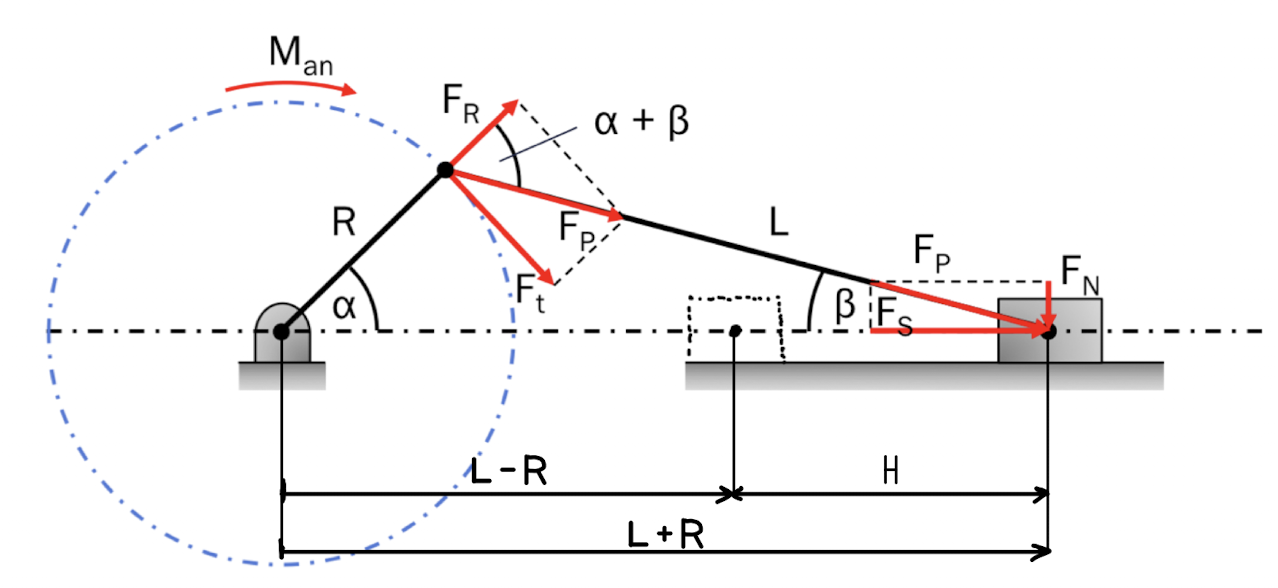
\includegraphics[width = 0.8\linewidth]{src/images/MAEIP_Schubkurbel}
        \begin{empheq}[box=\fbox]{align*}
            H = 2\cdot R \quad \mid \quad t = &\frac{1}{n} \quad \mid \quad \lambda = \frac{R}{L} = \frac{sin(\beta)}{sin(\alpha)}
            \\F_s = \frac{cos(\beta) \cdot M_{an}}{sin(\alpha + \beta) \cdot R} \quad &\mid \quad sin(\alpha + \beta) = \frac{F_t}{F_p}
            \\F_t = \frac{M_{an}}{R} \quad &\mid \quad cos(\beta) = \frac{F_s}{F_p}
        \end{empheq}
        $H$ = Hublänge; $t$ = Taktzeit (1x Hin und zurück); \\$\lambda$ = Schubstangenverhältnis (meist $0.1 \leq \lambda \leq 0.4$); $n$ = Drehzahl
    \end{center}
\end{footnotesize}

\subsubsection{Variation Kurbellänge \hfill IP}
\begin{footnotesize}
    \begin{center}
        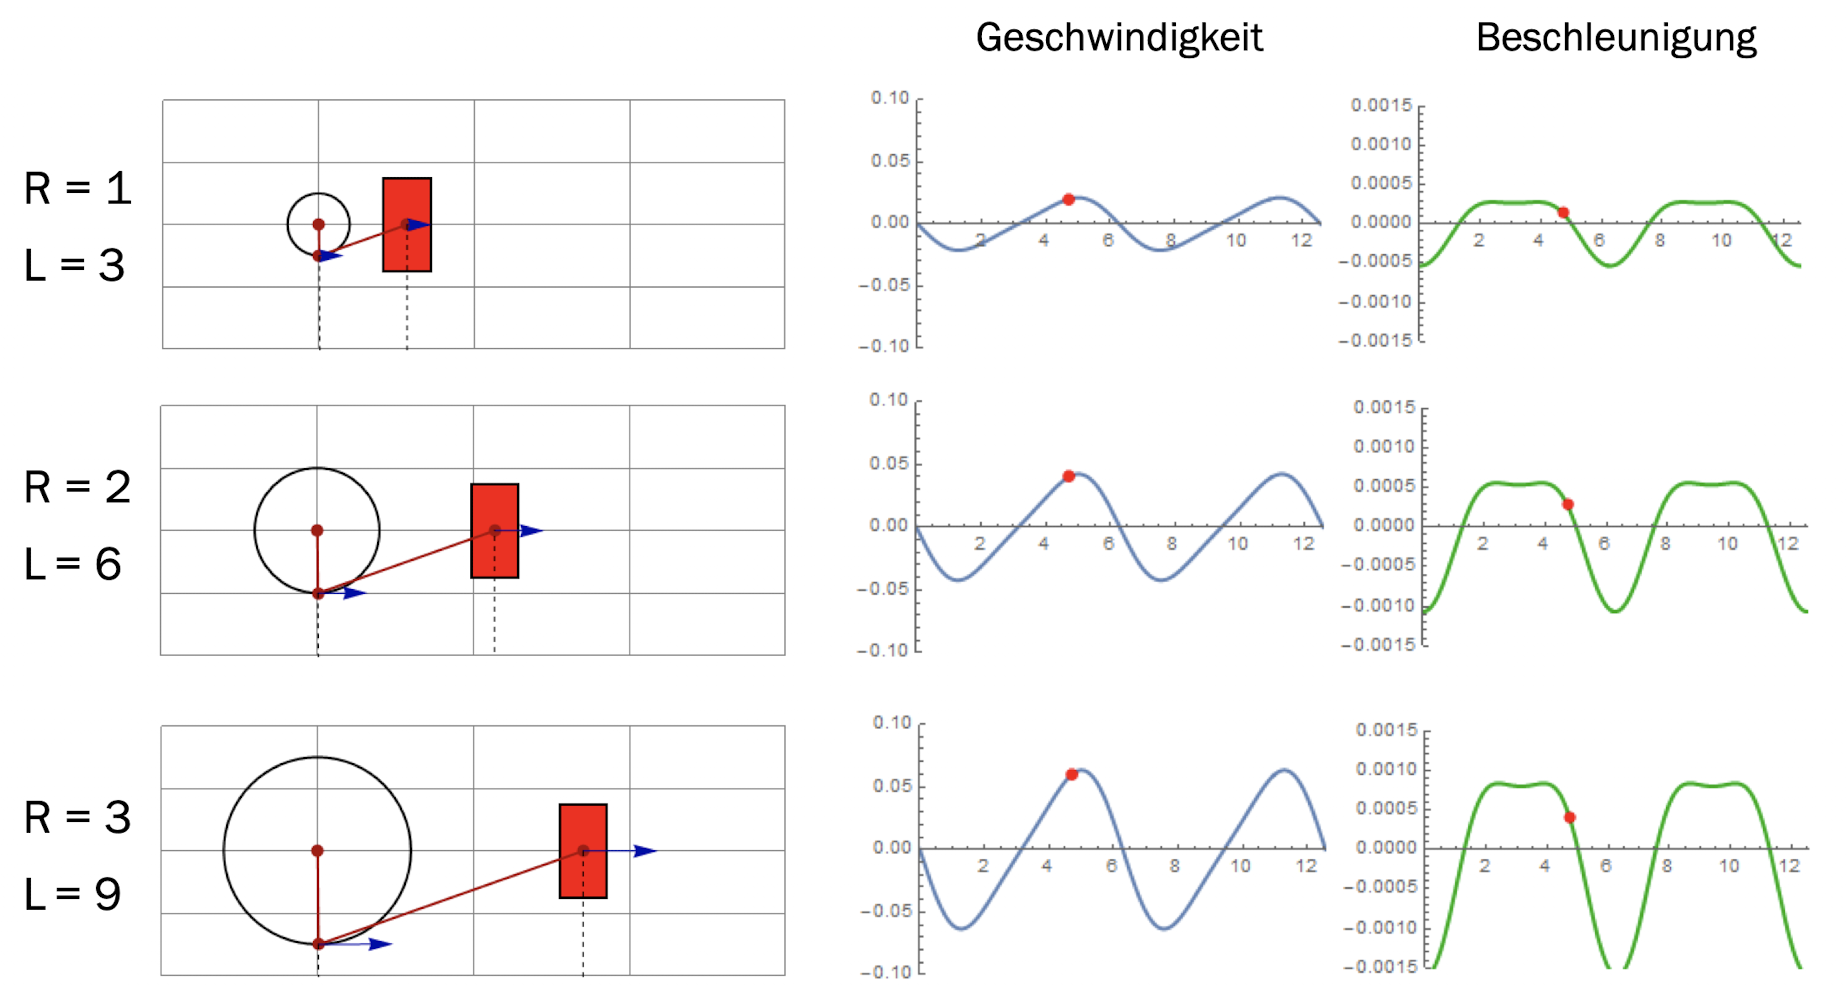
\includegraphics[width = 0.8\linewidth]{src/images/MAEIP_VariationKurbellaenge}
    \end{center}
    \begin{itemize}
        \item \textbf{Kurze Kurbel} $\to$ kleine Amplitude 
        \item \textbf{Lange Kurbel} $\to$ grosse Amplitude
        \item \textbf{Grosses Schubstangenverhältnis [R/L]} $\to$ Schwingung mit Senke
        \item \textbf{Kleines Schubstangenverhältnis [R/L]} $\to$ Schwingung ohne Senke
    \end{itemize}
\end{footnotesize}

\subsubsection{Variation Pleuellänge \hfill IP}
\begin{footnotesize}
    \begin{center}
        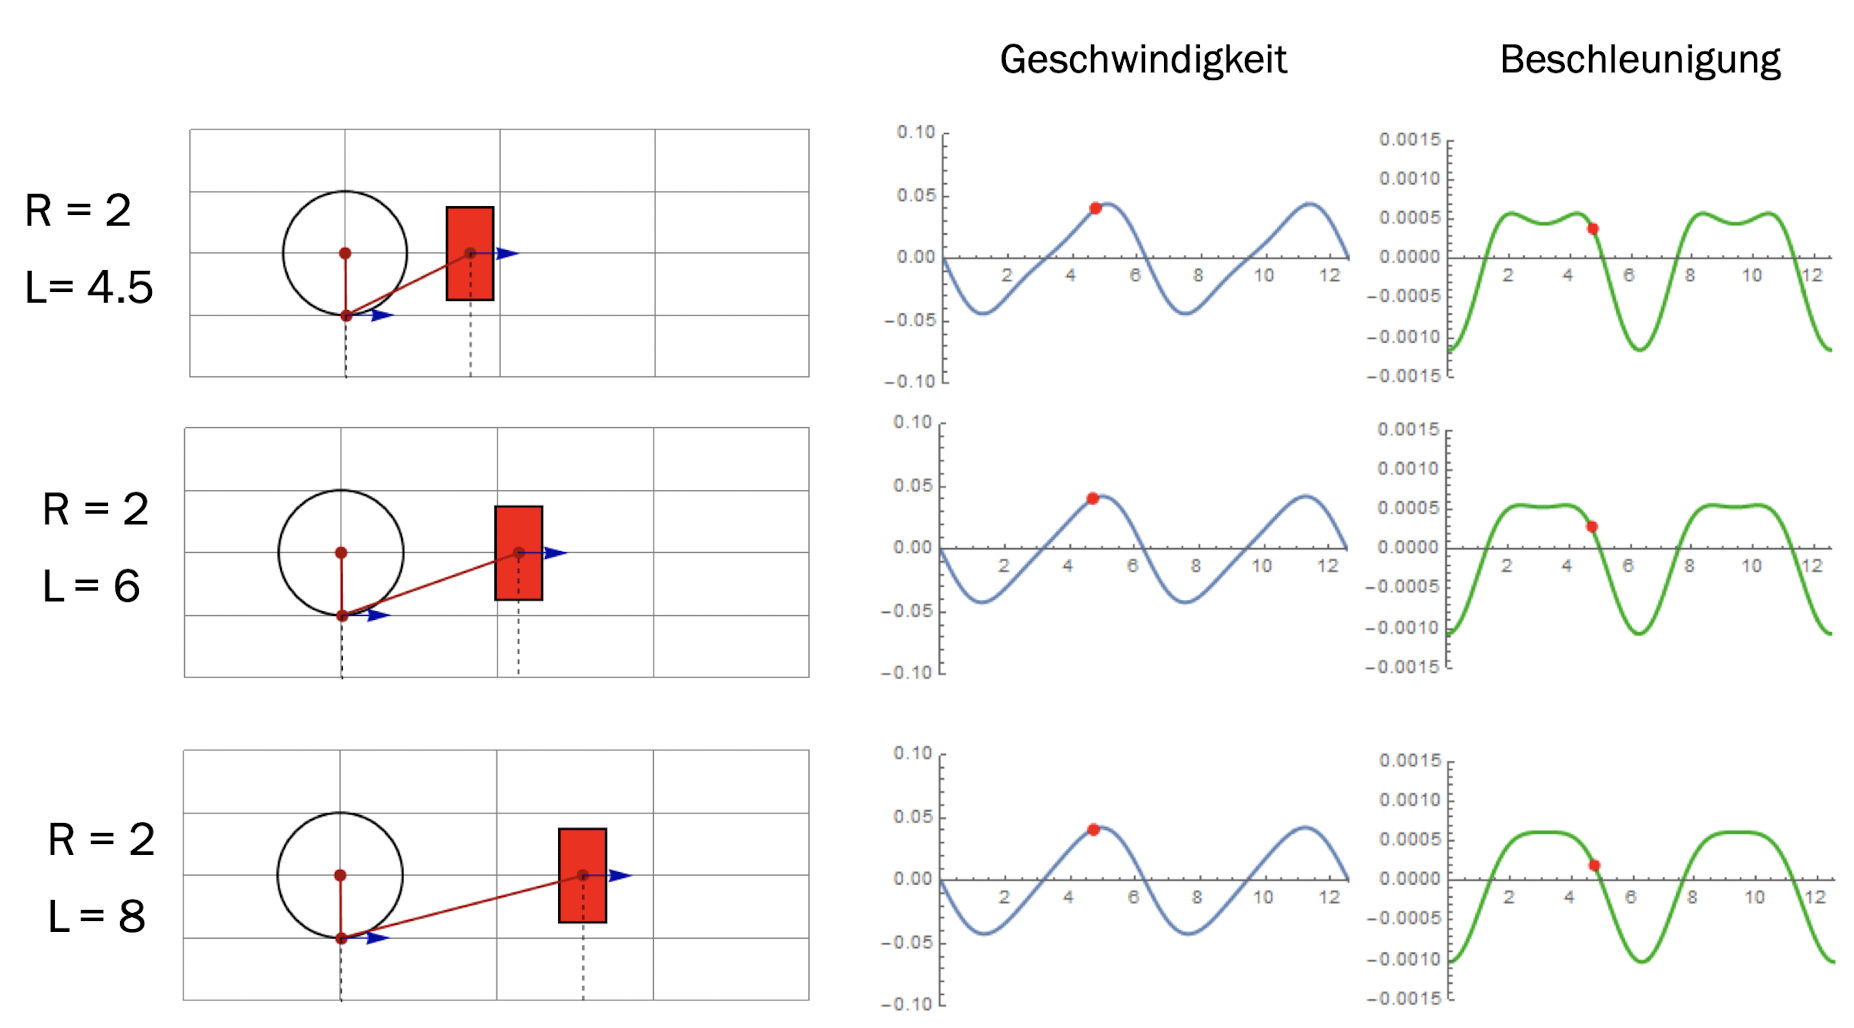
\includegraphics[width = 0.8\linewidth]{src/images/MAEIP_VariationPleuellaenge}
    \end{center}
\end{footnotesize}

\subsubsection{Kurbelschleife \hfill IP}
\begin{footnotesize}
    \begin{center}
        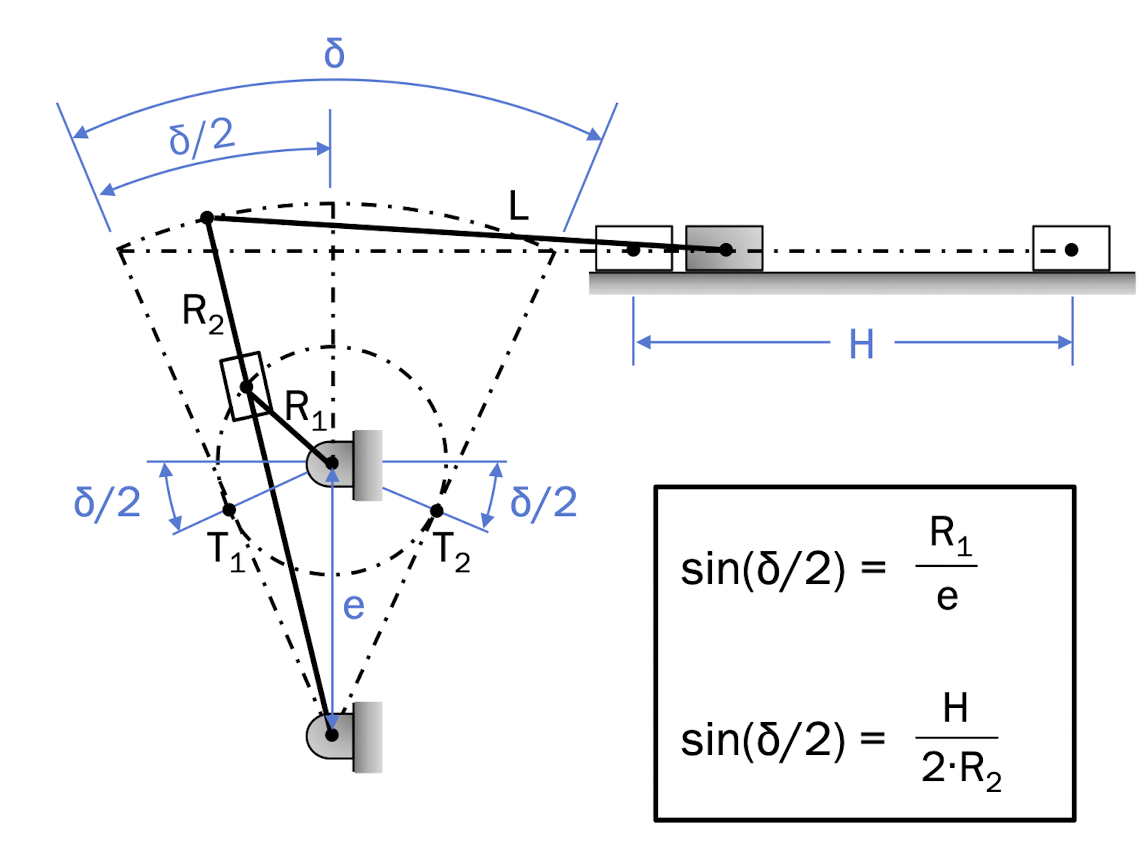
\includegraphics[width = 0.7\linewidth]{src/images/MAEIP_Kurbelschleife}
        \\Schubgelenk ist \textbf{nicht} Teil des Gestells
    \end{center}
\end{footnotesize}

\subsubsection{Exzentrische Schubkurbel \hfill IP}
\begin{footnotesize}
    \begin{center}
        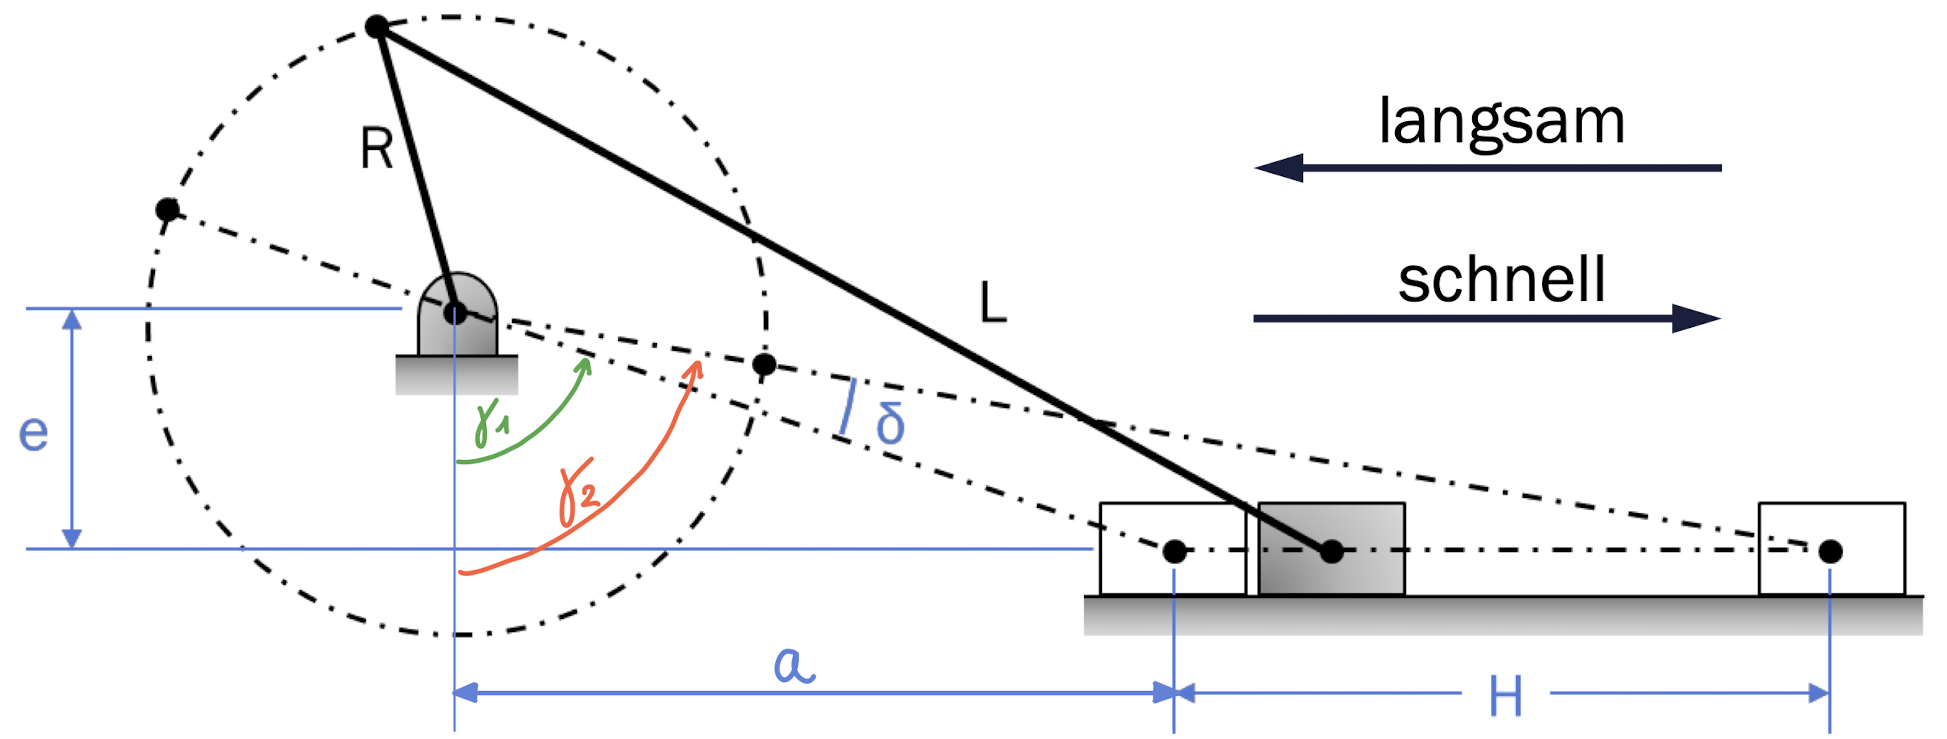
\includegraphics[width = 0.8\linewidth]{src/images/MAEIP_ExzentrischeKurbel}
        \begin{empheq}[box=\fbox]{align*}
            H &= \sqrt{(L+R)^2 - e^2} - \sqrt{(L-R)^2 - e^2} 
            \\a &= \sqrt{(L-R)^2 - e^2} \quad \mid \quad \delta = \gamma_2 - \gamma_1
            % \\cos(\delta) &= \frac{e^2 + \sqrt{\scriptstyle{(L^2-R^2)^2 - 2e^2(L^2+R^2) + e^4}}}{(L-R)^2}
            \\cos(\gamma_1) &= \frac{e}{(L-R)} \quad \mid \quad cos(\gamma_2) = \frac{e}{(L+R)}
            \\Q &= \frac{180^\circ + \delta}{180^\circ - \delta} \Rightarrow \delta = 180^\circ \cdot \frac{Q-1}{Q+1}
            \\t_{\text{hin}} &= \frac{60}{n(Q+1)} [s] \quad \mid \quad n \; [\text{min}^{-1}]
        \end{empheq}
        $Q$ = Zeitenverhältnis \\= (Zeit des langsamen Hubs / Zeit des schnellen Hubs)
    \end{center}
\end{footnotesize}